
% --------------------------------------------------------------
% This is all preamble stuff that you don't have to worry about.
% Head down to where it says "Start here"
% --------------------------------------------------------------

\documentclass[11pt]{article}

\usepackage{bera}
%\renewcommand{\familydefault}{\rmfamily}

\usepackage{graphicx,url}
\usepackage{proof}
\usepackage{framed}
\usepackage{etaremune}
\usepackage{graphics}

\usepackage[margin=1in]{geometry}
\usepackage{amsmath,amsthm,amssymb,amsfonts}
\usepackage{paralist}
\thispagestyle{empty}

% 1. To get version suitable for students to populate,
%    remove the contents of the \ignoreSoln{..body..}
%
% 2. To get a version suitable for generating PDF 
%    without solutions, remove the #1 below
%
% 3. To generate solutions, keep the #1 below
%
% 4. Assigned grader fills \ignoreSoln{..body..}
%    and also provides his/her feedback to student
%    and policy followed for point deduction
%    So design policy before grading begins.

\newcommand{\ignoreSoln}[1]{#1}   
%\newcommand{\ignoreModel}[1]{#1} 


\newcommand{\bigset}[2]{\big\{\;#1\;:\;#2\;\big\}}
\newcommand{\N}{\mathbb{N}}
\newcommand{\Z}{\mathbb{Z}}
\newcommand{\R}{\mathbb{R}}
\newcommand{\Np}{\mathbb{N^{+}}}

\newenvironment{theorem}[2][Theorem]{\begin{trivlist}
\item[\hskip \labelsep {\bfseries #1}\hskip \labelsep {\bfseries #2.}]}{\end{trivlist}}
\newenvironment{lemma}[2][Lemma]{\begin{trivlist}
\item[\hskip \labelsep {\bfseries #1}\hskip \labelsep {\bfseries #2.}]}{\end{trivlist}}
\newenvironment{exercise}[2][Exercise]{\begin{trivlist}
\item[\hskip \labelsep {\bfseries #1}\hskip \labelsep {\bfseries #2.}]}{\end{trivlist}}
\newenvironment{reflection}[2][Reflection]{\begin{trivlist}
\item[\hskip \labelsep {\bfseries #1}\hskip \labelsep {\bfseries #2.}]}{\end{trivlist}}
\newenvironment{proposition}[2][Proposition]{\begin{trivlist}
\item[\hskip \labelsep {\bfseries #1}\hskip \labelsep {\bfseries #2.}]}{\end{trivlist}}
\newenvironment{corollary}[2][Corollary]{\begin{trivlist}
\item[\hskip \labelsep {\bfseries #1}\hskip \labelsep {\bfseries #2.}]}{\end{trivlist}}

\DeclareMathSizes{14}{14}{14}{14}

\begin{document}

% --------------------------------------------------------------
%                         Start here
% --------------------------------------------------------------

%\renewcommand{\qedsymbol}{\filledbox}
\newlength{\minpagw}
\settowidth{\minpagw}{\hspace{40em}}

\begin{center}
\begin{large}
  CS 6110, Spring 2022, Assignment 5  \\
  Given 2/22/22 -- Due 3/3/22 by 11:59 pm via your Github 
  \ \\
%  \ \\  
    {  {\Large\bf NAME: Tripti Agarwal} \hfill {\Large\bf UNID: u1319433}\hspace{4cm} }
          \ \\
\end{large}

\end{center}


\begin{enumerate}

%- 1 ----------------------------------------------------------------
\item (10 points)
  \textbf{Read and summarize Jackson's article on Alloy}


  
\begin{minipage}{\minpagw}
  \fbox{%
    \parbox{\linewidth}{%
      Alloy tool can be used to explore models that arise in different software design. We can use simple logic relation in alloy to build structures that are dependent on relations. We can simulate designs and find flaws in our structure using alloy as it uses SAT technology. It is complementary to model checking tools.
      \begin{itemize}
          \item The software we design should have the properties we expect. Informal representation give inconsistent interpretations and they cannot be analysed easily. By using formality, we can minimize the cost of ambiguity and can get quicker feedbacks.
          \item Theorem provers are mechanical aids for constructing mathematical proofs. We need expressive logic and sound proofs which are hard to automate. Hence a lot of effort and expertise id required for this process.
          \item Model checker provides push-button automation, and the user have to just provide the design and property that needs to be checked. They provide counter examples when properties are not true. They also allow dynamic properties to be expressed. But model checkers have a problem of state explosion.
          \item Alloy is built to provide the advantages  and eliminate the problems of model checker. Model checkers are used for parallelism and simple states, but do not provide support for rich structures like trees, lists, tables and graphs. 
      \end{itemize}
      Alloy innovations
      \begin{itemize}
          \item Relational logic are used in alloy for both describing designs and properties.
          \item Alloy incorporated the power of Z language in which the sets and relations are used for software design.
          \item Alloy allows only first order structures, thus ruling out sets over sets and relations  over sets.
          \item The key operator us relational join, which works with relations of any arity. With alloy we can describe the universe of objects as a classification of tree. Alloy runs all small tests. The designer can specify the scope that bounds for each of the specifications given. Alloy translates the design problem to a satisfiability problem whose variables are not relations but simple bits.
      \end{itemize}}%
  }%
\end{minipage}  

\begin{figure}
\begin{minipage}{\minpagw}
  \fbox{%
    \parbox{\linewidth}{%
      How to use alloy analyser and an example
      \begin{itemize}
          \item A structure is represented as a signature "sig" which can be a collection of points and we can also specify the property that these points can hold. For example in the screenshot we see two signature EndPoint and HTTPEvent. The HTTPEvent consists of collection of points to and from. The run command will execute to produce an instance of the httpevent that has been created.\\
          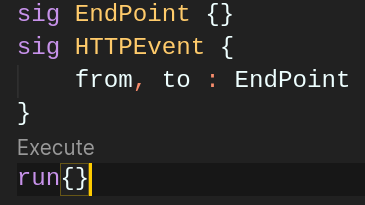
\includegraphics[width=2.0in]{q1_1.png}
          \item We can further classify the EndPoints as clients and servers. The HTTPEvents are also classified as requests and response to obtain a graph that shows the connection between clients, servers, response and request.\\
          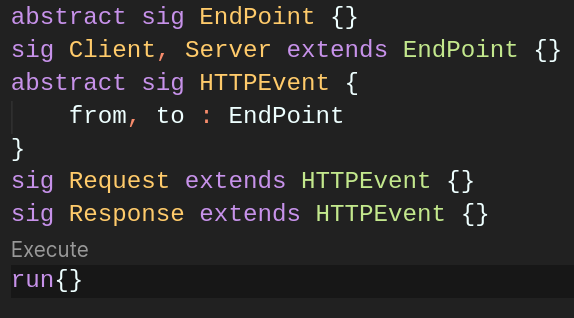
\includegraphics[width=2.0in]{q1_2.png}
          \item We can improve the theme in alloy by giving different colors to each object and the relations. The figure below shows the martha palette in the theme and giving different colors by changing the general graph settings.\\
          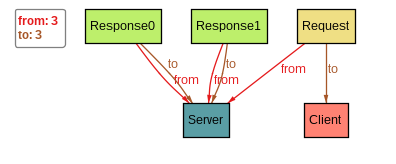
\includegraphics[width=2.0in]{q1_3.png}
          \item We see in the above figure that the request is to the server and response is to and from server. This can be constrained by using a fact as shown the figure below.\\
          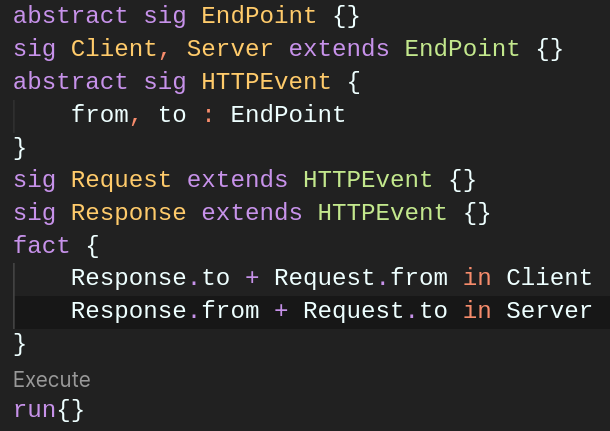
\includegraphics[width=3.0in]{q1_4.png}
      \end{itemize}
    }%
  }%
\end{minipage}  
\end{figure}
\begin{figure}
   
\begin{minipage}{\minpagw}
  \fbox{%
    \parbox{\linewidth}{%
      \begin{itemize}
          \item To create a relation between request and response, we set a property in the reponse to point out how request is related to response. To obtain exactly one response for each request we set a fact that each response is for exactly one request. We can also add a constraint of each property that we want to see in the run command.
           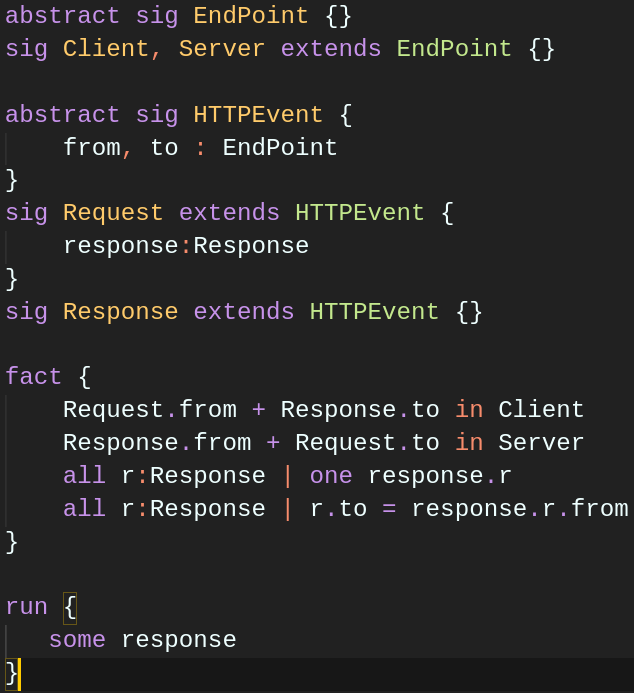
\includegraphics[width=3.0in]{q1_5.png}
           \item To see if any property is true for our model, we use check command. For example we can check that any request if to goes as the reponse to the same request it originally comes from. If the alloy finds a counter example then the claimed property does not exactly hold. This means we need to constraint out facts again. Once the facts are all fixed then the check will not produce any counter example.
           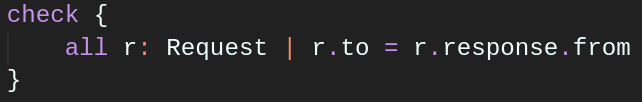
\includegraphics[width=3.0in]{q1_6.png}
           \item If alloy produce no counter example then produce the core for the model. The core produce the instance that are used to check the property that has been provided.
           \end{itemize}
    }%
  }%
\end{minipage}  
\end{figure}
\newpage
%- 2 ----------------------------------------------------------------
\item (25 points)
  \textbf{Take the tutorial on
  \url{https://www.doc.ic.ac.uk/project/examples/2007/271j/suprema_on_alloy/Web/index.php}}
 \begin{figure}
     

\begin{minipage}{\minpagw}
  \fbox{%
    \parbox{\linewidth}{%
     \begin{itemize}
         \item \textbf{Statics I} The tutorial is to use alloy to model the implementation of a Queue. Every queue has a root node and a reference to next node in the queue. We decalre two signatures in the alloy one for the queue and other for the node. The queue consists of the root which is a lone Node and the node consists of next which is also a type of lone Node. Lone means zero or one. To produce any instance of the Queue we can use predicate with no constraints. To get samples of predicate we use run command. We can force the run command to produce instance of a particular size. We can add facts to constrain our model. 
         \item \textbf{Statics II} The $*$ operator represents the reflexive transitive closure. The operator $\Hat{}$ (hat) is use to represent non-reflexive transitive closure. Ally provides us the facility to visualize different instances of the model to find errors. This helps us in substituting specific constraint to obtain the correct model.
         \item \textbf{Dynamics I} Abstract ensures that there cannot be direct instances of the object. In the predicate we can constraint what type of instances to produce. We use $\#$ to produce number of any type of signature. Exactly is to constraint a particular number of instance to produce.We can use assert to restrict the model to have a particular assertion. We can then check the assertion to see if the model produces an output or not. If yes then the model is not correct otherwise the model follows the assertion. All is used for the all the elements in the set and some for some elements in the set.
         \item \textbf{Dynamics II} + is a set union operator. This means that the set of values after is equal to the union of the set of values before with extra mapping from k to v. fun is used to create a function in alloy and arguments to a function are enclosed in square brackets. Dot (.) operator is used to return all values that are associated with a particular object.
         \item \textbf{Evidence of the test} 

            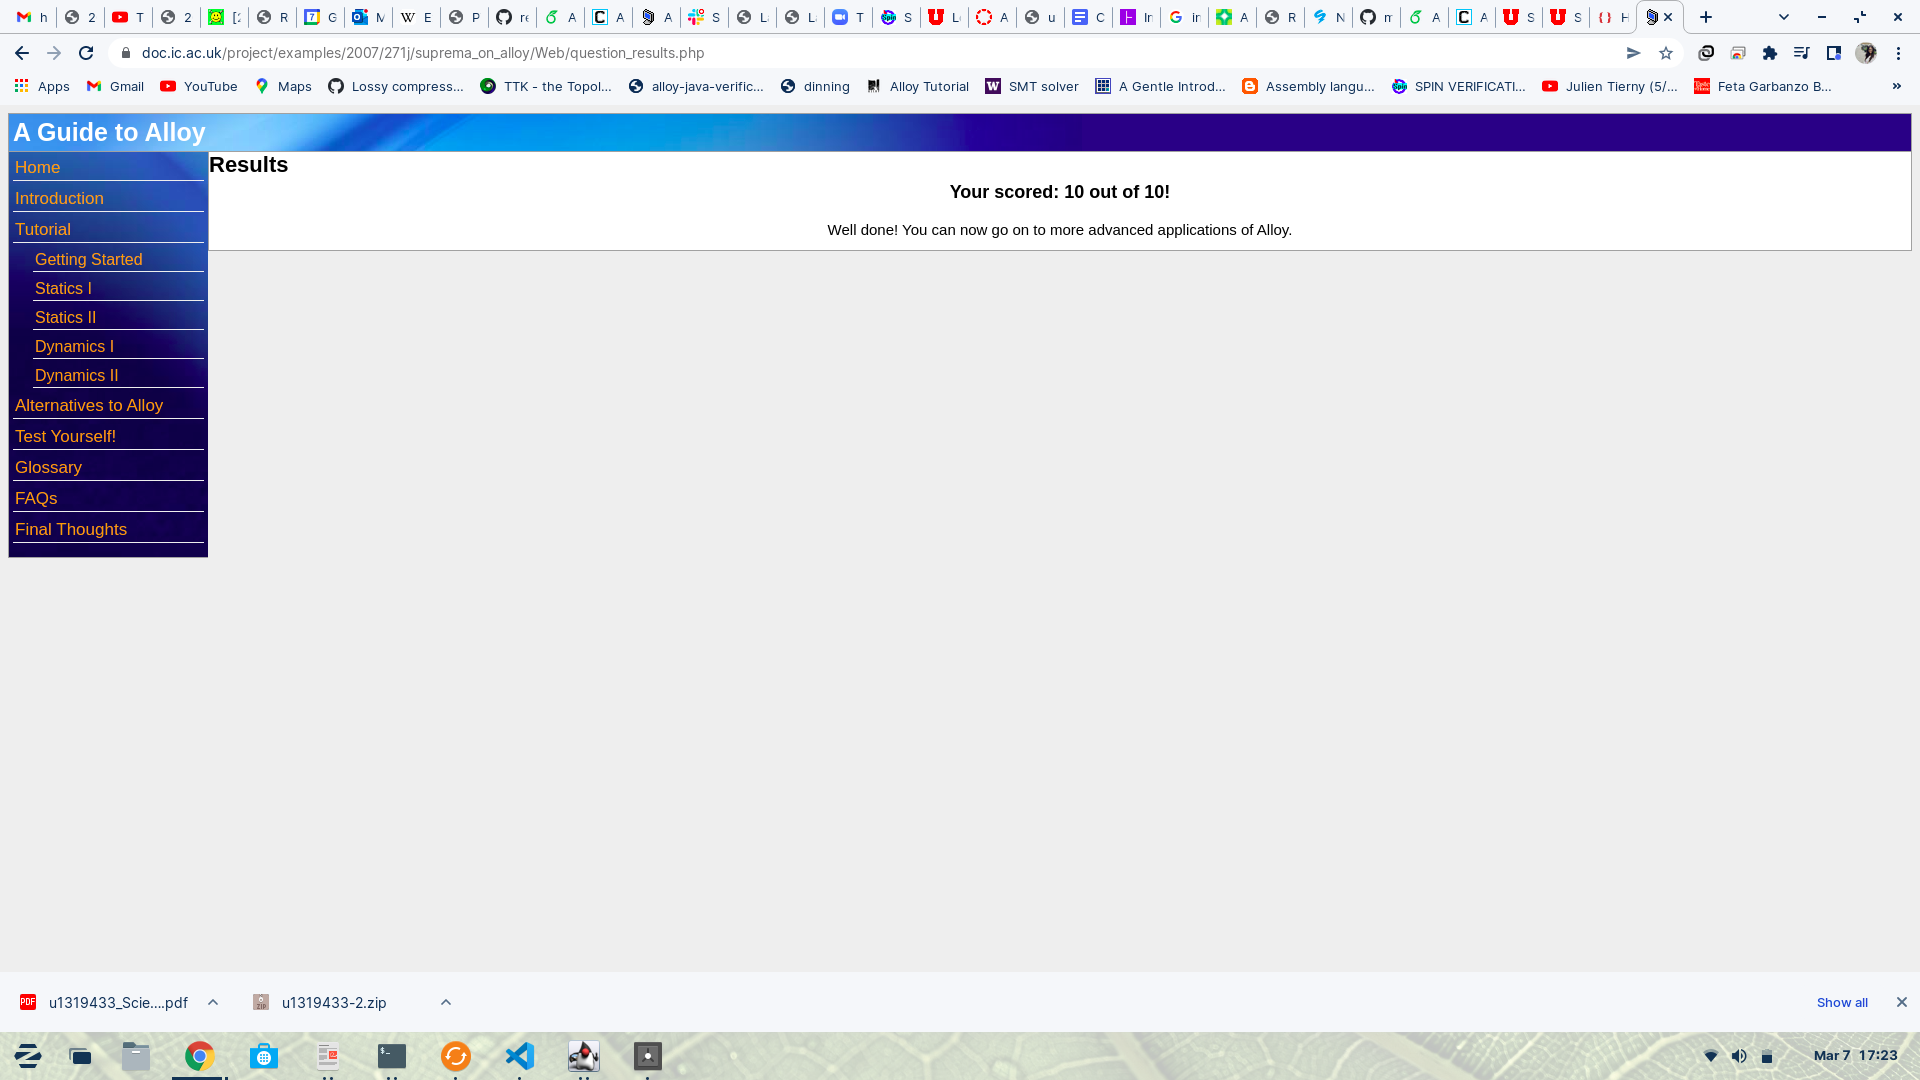
\includegraphics[width=3.0in]{Q2.png}
    
     \end{itemize}
    }%
  }%
  \end{minipage}
   \end{figure} 
 \newpage
%- 3 ----------------------------------------------------------------
\item (40 points)
  First, deep-read the Alloy ``Red book'' linked on the class website
  from the beginning till Page 80.
  Summarize the concepts you find on these pages in four pages.
  Thus, there are three tree models below.
  %
  Study them and do the problems stated below them:


\begin{itemize}
\item[] 
\textbf{Q1 :  no node in the tree that points to the root}\\
\textbf{Q2 :  no node in the tree that points to another node such that it makes a loop (non-transitive)}
\\
We cannot use $*$ because this means reflexive transitive closure, whereas $\hat{.}$ means transitive closure. If we use $*$, it will make nodes point to itself. No instances are found if we use $*$ instead of $\hat{.}$



\item[] 
\textbf{Q3 : all the nodes except the root has a root, there is only one root and the tree is one connected tree.}\\ We need Node - root so that the relation applied is not applied to the root. Hence there is no root for the root node.
\item[] 
\textbf{Q4 : no node points to itself (non-reflexive).}\\
If we leave disj then we end up getting just one root node. This is because all the properties are too strict and hence we just get a tree consisting of only one node.


\item[]
\textbf{Q5 :no transitive relation between nodes}
\begin{enumerate}
\item Issue \verb|check {GGTree iff DJTree} for 5| and see if the definitions are equivalent.\\
\textbf{Since no instances are found, hence the two definitions, GGTree and DJTree are equivalent}
\item Just break the Q-1 to have \verb|*| and not the correct \verb|^|. Do the ``\verb|iff|''  check above.
Do you get an understandable counterexample? Describe it.\\
\textbf{After breaking the $*$ in Q1, we end up getting counter examples. This means that there is a reflexive relation between the nodes and they can point to the root. Such a tree is not possible and hence we end up getting counter examples that does not exists in GGTree but exists in DJTree.}
\item Issue \verb|check {CostelloTree iff DJTree} for 5| and see if the definitions are equivalent.\\
\textbf{Since no instances are found, hence the two definitions, CostelloTree and DJTree are equivalent}
\\
The codes are available on Github as tree.als and broken\_tree.als
\end{enumerate}

\end{itemize}
  
\begin{minipage}{\minpagw}
  \fbox{%
    \parbox{\linewidth}{%
    \begin{itemize}
        \item Some issues might look trivial and are not easy to identify. Alloy provides you the facility to get a graphical representation of the system consisting of nodes and edges, defined over different functions to show the relationship.
        \item In alloy model, signatures are used which consists of objects. We can map any of the objects by using a field name and then defining a relationship that exists on it. Keywords like lone can be used to show multiplicity.
        \item Predicate and run commands are used to find the instance of the possible states. We can use use the pound  to show the instance of a particular link constraint to a specific number.
        \item Different dynamic operators like add can be used to produce a specific constraint. Even though Alloy is declarative, it can still be executed like operational language. This is done using the run command. 
        \item Other dynamic operations are minus (-), dot (.). - is used for deletion and . can be used to find a particular object in a signature.
        \item Assert is used to insert an assertion. To check the assertion we use check command. If we get a counter example then the assertion is not valid.
        \item We can create alias for an object in Alloy. This is done using extends keyword. The hat  operator is used for transitive closure. We can write facts that are true for signatures.
        \item We can create functions using keyword fun. Overall, alloy do not use any unfamiliar or complicated mathematics and it is easy to these symbols as these are based on simple basic logic and a special dot operator for navigate along relations, which is similar to deferencing in java.
        \item We can write partial description of any operation that allows different behaviours.
        \item With assertions we can test everything and we do not need any extra test case to check the results.
        \item Navigation expressions are commonly used as multiplicity constraints are very common. The predicate calculus is commonly used in comprehension expressions. These are also used when writing concrete and straightforward constraints.
        \item Relational calculus are used for some commonly recurring constraints that can be expressed more concisely, example no $\hat{}r \&$ iden to say that the relation r is acyclic.
        \item An atom is a primitive entity that is indivisible, immutable, and uninterpreted.
        
        
    \end{itemize}
    }%
  }%
\end{minipage}  
\newpage
\begin{minipage}{\minpagw}
  \fbox{%
    \parbox{\linewidth}{%
    \begin{itemize}
\item A relation is a structure that relates atoms. It consists of a set of tuples, each tuple being a sequence of atoms. A relation can have any number of rows, called its size. Any size is possible, including zero. The number of columns in a relation is called its arity, and must be one or more. Relations with arity one, two, and three are said to be unary, binary, and ternary. A relation with arity of three or more is a multirelation.
        \item A unary relation with only one tuple, corresponding to a table with a single entry, represents a scalar. A relation with no tuples is empty. A unary relation with at most one tuple—that is, a relation that is either a scalar or empty—is called an option.
        \item Composite objects can be created with atoms for the components and a relation to bind them together. We can model mutation, in which the value of an object changes over time, by separating the identity of the object and its value into separate atoms, and relating identities, values and times.
        \item Atom names never appear in models; they’re only used to describe instances produced by simulation or checking. All structures are relations, and a set is simply a relation all of whose tuples contain only one element. The restriction to flat relations makes the logic more tractable for analysis.
        \item There is a loss of expressive power in the restriction to flat relations, which can be work around. Relations have finite size and arity. Multirelations are used because relations are flat rather than nested, arities greater than two are very common. To model execution traces of a system whose state involves relationships will require ternary relations: two columns for the relationship at a given time, and an additional column for the time.
        \item An unordered relationship can be represented in different ways. The simplest way is to use a relation r (ordered, as always), and add a constraint r = $\tilde{r}$ that makes it symmetric—the same forward and backward.
        \item A binary relation that maps each atom to at most one other atom is said to be functional, and is called a function. A binary relation that maps at most one atom to each atom is injective.
        \item The domain of a relation is the set of atoms in its first column; the range is the set in the last column.
        \item Particular values of sets and binary relations can be shown graphically in a snapshot. Alloy creates a node for each atom, and draw an arc for each tuple connecting the nodes corresponding to the first and second atoms in the tuple. To show several relations, you label each tuple arc with the relation it belongs to. Sets can be shown in two ways: either by an extra label in a node naming a set it belongs to, or by drawing a labelled contour around some nodes.
\end{itemize} 
    }%
  }%
\end{minipage}  
\newpage
\begin{minipage}{\minpagw}
  \fbox{%
    \parbox{\linewidth}{%
    \begin{itemize}
    \item Multirelations can be shown as graphs by projecting out one or more columns. Projection takes two steps. Suppose just one column is being projected out. In the first step, the column is moved to the front, so that it becomes the first column of the relation; each tuple is permuted accordingly. In the second step, the relation is split into an indexed collection of relations. For each atom that appears in the first column, we associate the relation consisting of all those tuples that begin with that atom, but with the atom removed.
    \item There are three constants: none, univ and iden. None and univ , represents the set containing no atom and every atom respectively, are unary. To denote the empty binary relation, we can write none $\rightarrow$ none , and for the universal relation that maps every atom to every atom, univ $\rightarrow$ univ. The identity relation is binary, and contains a tuple relating every atom to itself.
    \item The set operators are $+$ (union), $\&$ (intersection), $-$ (difference), in (subset), $=$ (equality). These operators can be applied to any pair of relations so long as they have the same arity. Because scalars are just singleton sets, the braces used to form sets from scalars in traditional mathematical notation aren’t needed.
    \item The relational operators are : $\rightarrow$ (arrow - product), $.$ (dot- join), $[]$ (box- join), $\tilde{}$ (transpose), $\hat{.}$ (transitive closure), * (reflexive-transitive closure) $<:$ (domain restriction), $:>$ (range restriction), $++$ (override).
    \item The arrow product (or just product) p $\rightarrow$ q of two relations p and q is the relation you get by taking every combination of a tuple from p and a tuple from q and concatenating them.
    \item The quintessential relational operator is composition, or join. The dot join (or just join) p.q of relations p and q is the relation you get by taking every combination of a tuple in p and a tuple in q , and including their join, if it exists.
    \item The transpose $\tilde{.}$r of a binary relation r takes its mirror image, forming a new relation by reversing the order of atoms in each tuple.
    \item A binary relation is transitive if, whenever it contains the tuples a $\rigtharrow$ b and b $\rigtharrow$ c , it also contains a $\rigtharrow$ c , or more succinctly as a relational constraint: r$.$r in r. The transitive closure $\hat{.}$r of a binary relation r , or just the closure for short, is the smallest relation that contains r and is transitive.
    \item The restriction operators are used to filter relations to a given domain or range. The expression s $<:$ r , formed from a set s and a relation r , contains those tuples of r that start with an element in s . Similarly, r $:>$ s contains the tuples of r that end with an element in s . Restrictions can be applied to relations of any arity of two or more, but are most often applied to binary relations.
\end{itemize} 
    }%
  }%
\end{minipage} 
\newpage
\begin{minipage}{\minpagw}
  \fbox{%
    \parbox{\linewidth}{%
    \begin{itemize}
    
    \item The override p $++$ q of relation p by relation q is like the union, except that the tuples of q can replace the tuples of p rather than just augmenting them. Any tuple in p that matches a tuple in q by starting with the same element is dropped. The relations p and q can have any matching arity of two or more.
    \item Operators have a standard precedence ranking so that constraints aren’t marred by masses of parentheses. The ranking follows the usual conventions: unary operators (closure, transpose) precede binary operators; product operators (such as dot and arrow) precede sum operators (plus, minus, intersect).
    \item We’ve seen how to make a constraint from two expressions using the comparison operators in and = . Larger constraints are made from smaller constraints by combining them with the standard logical operators and by quantifying constraints that contain free variables over bindings.
    \item There are two forms of each logical operator: a shorthand and a verbose form: not (negation), and (conjunction), or (disjunction), implies (implication), else (alternative), iff (bi-implication).
    \item A quantified constraint takes the form Q x: e | F where F is a constraint that contains the variable x , e is an expression bounding x , and Q is a quantifier. Quantifiers in alloy: all, some, no, lone, one.
    \item When an expression appears repeatedly, or is a subexpression of a larger, complicated expression, you can factor it out. The form let x = e | A is short for A with each occurrence of the variable x replaced by the expression e . The body of the let, A , and thus the form as a whole, can be a constraint or an expression. 
    \item Comprehensions make relations from properties. A declaration introduces a relation name. A constraint of the form relation-name : expression is called a declaration. Multiplicities are expressed with the multiplicity keywords: set, one, lone, some.
    \item Suppose the declaration looks like this: r: A m $\rightarrow$ n B where m and n are multiplicity keywords (and where A and B are, for now, sets). Then the relation r is constrained to map each member of A to n members of B , and to map m members of A to each member of B.
    \item Declarations usually introduce new names, but they can also be used to impose constraints on relations that have already been declared, or on arbitrary expressions.
    \item Multiplicities can be nested. Suppose you have a declaration of the form r: A $\rightarrow$ (B m $\rightarrow$ n C) This means that, for each tuple in A , the corresponding tuples in B $\rightarrow$ C form a relation with the given multiplicity.
    \item The operator pound applied to a relation gives the number of tuples it contains, as an integer value. The following operators can be used to combine and compare integers: +, -, =, <, >, =<, >=.
    \end{itemize} 
    }%
  }%
\end{minipage} 
\newpage
%- 2 ----------------------------------------------------------------
\item (25 points) Write your own quicksort and broken quicksort in C with klee assertions 
\begin{figure}[!h]
  \begin{minipage}{\minpagw}
  \fbox{%
    \parbox{\linewidth}{%
      The code is available on Github quicksort.c and broken\_quicksort.c.
      Here is the output screenshot for quicksort and its broken version (as decribed in the question)\\
      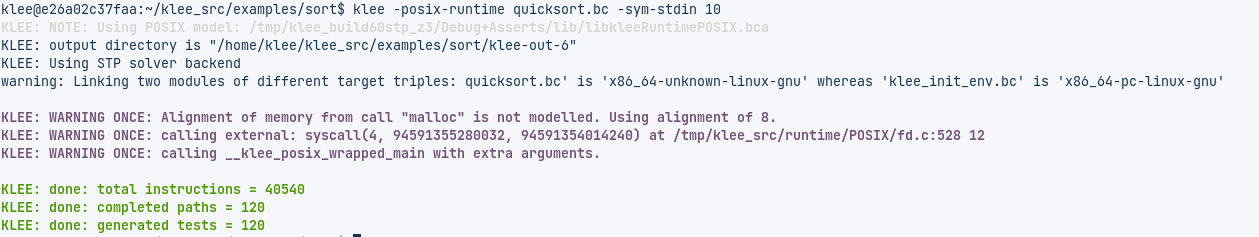
\includegraphics[width=5.8in]{quicksort.png}
    \caption{Klee output for quicksort.c}
    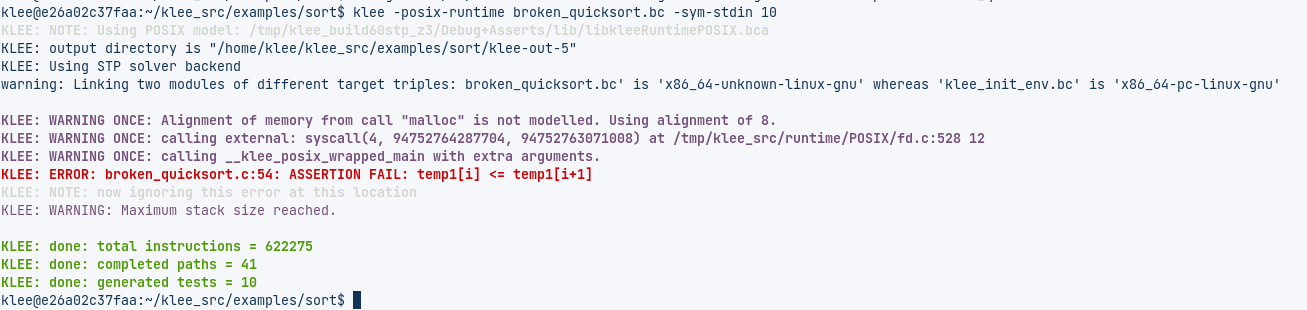
\includegraphics[width=5.8in]{broken_qsort.png}
    \caption{Klee output for broken\_quicksort.c}
    
    }%
  }%
  \end{minipage}
\end{figure}
  
  
%- end ----------------------------------------------------------------  


\end{enumerate}

\end{document}
